\documentclass{sigchi}

% Use this section to set the ACM copyright statement (e.g. for
% preprints).  Consult the conference website for the camera-ready
% copyright statement.

% Copyright
%\CopyrightYear{2020}
%\setcopyright{acmcopyright}
%\setcopyright{acmlicensed}
%\setcopyright{rightsretained}
%\setcopyright{usgov}
%\setcopyright{usgovmixed}
%\setcopyright{cagov}
%\setcopyright{cagovmixed}
% DOI
%\doi{https://doi.org/10.1145/3313831.XXXXXXX}
% ISBN
% \isbn{978-1-4503-6708-0/20/04}
%Conference
\conferenceinfo{CHI'20,}{April  25--30, 2020, Honolulu, HI, USA}
%Price

% Use this command to override the default ACM copyright statement
% (e.g. for preprints).  Consult the conference website for the
% camera-ready copyright statement.

%% HOW TO OVERRIDE THE DEFAULT COPYRIGHT STRIP --
%% Please note you need to make sure the copy for your specific
%% license is used here!
% \toappear{
% Permission to make digital or hard copies of all or part of this work
% for personal or classroom use is granted without fee provided that
% copies are not made or distributed for profit or commercial advantage
% and that copies bear this notice and the full citation on the first
% page. Copyrights for components of this work owned by others than ACM
% must be honored. Abstracting with credit is permitted. To copy
% otherwise, or republish, to post on servers or to redistribute to
% lists, requires prior specific permission and/or a fee. Request
% permissions from \href{mailto:Permissions@acm.org}{Permissions@acm.org}. \\
% \emph{CHI '16},  May 07--12, 2016, San Jose, CA, USA \\
% ACM xxx-x-xxxx-xxxx-x/xx/xx\ldots \$15.00 \\
% DOI: \url{http://dx.doi.org/xx.xxxx/xxxxxxx.xxxxxxx}
% }

% Arabic page numbers for submission.  Remove this line to eliminate
% page numbers for the camera ready copy
% \pagenumbering{arabic}

% Load basic packages
\usepackage{balance}       % to better equalize the last page
\usepackage{graphics}      % for EPS, load graphicx instead 
\usepackage[T1]{fontenc}   % for umlauts and other diaeresis
\usepackage{txfonts}
\usepackage{mathptmx}
\usepackage[pdflang={en-US},pdftex]{hyperref}
\usepackage{color}
\usepackage{booktabs}
\usepackage{textcomp}


% Some optional stuff you might like/need.
\usepackage{microtype}        % Improved Tracking and Kerning
% \usepackage[all]{hypcap}    % Fixes bug in hyperref caption linking
\usepackage{ccicons}          % Cite your images correctly!
% \usepackage[utf8]{inputenc} % for a UTF8 editor only

% If you want to use todo notes, marginpars etc. during creation of
% your draft document, you have to enable the "chi_draft" option for
% the document class. To do this, change the very first line to:
% "\documentclass[chi_draft]{sigchi}". You can then place todo notes
% by using the "\todo{...}"  command. Make sure to disable the draft
% option again before submitting your final document.
\usepackage{todonotes}

% Paper metadata (use plain text, for PDF inclusion and later
% re-using, if desired).  Use \emtpyauthor when submitting for review
% so you remain anonymous.
\def\plaintitle{The Far Journey}
\def\plainauthor{First Author, Second Author, Third Author,
  Fourth Author, Fifth Author, Sixth Author}
\def\emptyauthor{}
\def\plainkeywords{Authors' choice; of terms; separated; by
  semicolons; include commas, within terms only; this section is required.}
\def\plaingeneralterms{Documentation, Standardization}

% llt: Define a global style for URLs, rather that the default one
\makeatletter
\def\url@leostyle{%
  \@ifundefined{selectfont}{
    \def\UrlFont{\sf}
  }{
    \def\UrlFont{\small\bf\ttfamily}
  }}
\makeatother
\urlstyle{leo}

% To make various LaTeX processors do the right thing with page size.
\def\pprw{8.5in}
\def\pprh{11in}
\special{papersize=\pprw,\pprh}
\setlength{\paperwidth}{\pprw}
\setlength{\paperheight}{\pprh}
\setlength{\pdfpagewidth}{\pprw}
\setlength{\pdfpageheight}{\pprh}

% Make sure hyperref comes last of your loaded packages, to give it a
% fighting chance of not being over-written, since its job is to
% redefine many LaTeX commands.
\definecolor{linkColor}{RGB}{6,125,233}
\hypersetup{%
  pdftitle={\plaintitle},
% Use \plainauthor for final version.
%  pdfauthor={\plainauthor},
  pdfauthor={\emptyauthor},
  pdfkeywords={\plainkeywords},
  pdfdisplaydoctitle=true, % For Accessibility
  bookmarksnumbered,
  pdfstartview={FitH},
  colorlinks,
  citecolor=black,
  filecolor=black,
  linkcolor=black,
  urlcolor=linkColor,
  breaklinks=true,
  hypertexnames=false
}

% create a shortcut to typeset table headings
% \newcommand\tabhead[1]{\small\textbf{#1}}

% End of preamble. Here it comes the document.
\begin{document}

\title{\plaintitle}

\numberofauthors{2}
\author{%
  \alignauthor{James Blankenship\\
    \affaddr{for Submission}\\
    \affaddr{Crockett Mills, US}\\
    \email{jamcblan@ut.utm.edu}}\\
  \alignauthor{Andrew Marshall\\
    \affaddr{for Submission}\\
    \affaddr{Martin, US}\\
    \email{jesamars@ut.utm.edu}}\\
  }

\maketitle

\begin{abstract}
  UPDATED---\today. Our project is a 3D real time game in the Unreal engine. 
  The game is a fantasy genre in a medieval setting. The game will have 3 levels in it.
  It will have a variety of enemies and weapons. There will be magic. The different types of magic for the player to use would include pyromancy and sorcery.There will be a class system that has two classes.The two classes are the Mage and the Warrior. Each level will have a boss enemy in it.
   \end{abstract}


% Author Keywords
\keywords{\plainkeywords}



\section{Introduction}
To introduce this project we decided to develop a game, and  the game will have the title of  "The Deep Journey." This game is in the first person. The general setting is that of medieval fantasy, and it will have 3 different levels  The first level will be where the character will start out in, and it will be the castle level. The castle  includes two  courtyards and middle building. The second level will be the castles dungeon which will have holding cells for enemies and middle room where the main boss is.The third level will be the fort  area which will be a walled structure with small buildings.The main building for the level will be a tavern which will hold the boss. The character player will have different type of weapons to choose from which will include hammer or staffs . The character player will be facing off against different enemies types including orcs, and wolves.  The character will also be able to wield different kinds of magic. There will be two different types of magic the character can wield pyromancy and sorcery.  


\section{Technical specifications}
We are using Unreal Engine for our project. We will be using C++ and blueprints in Unreal and behavior trees for the AI. Behavior trees are essentially used to create AI by having branches that decide actions.1 Blueprints will be used in places that require simple execution such as taking the player to a new level. An example would be the AI just searching and then it will execute a different branch when it finds someone. GitHub is being used for collaboration with each other and version control. All the assets that are currently being used is in the unreal store. 
\section{Levels}
There are three levels in this game.The first is the castle area and it was the first one made.It is two court yard and a main building each courtyard will have some smaller enemies for you to deal with.The Middle building will have two stories.The first one is just a way to get to the other court yard,basement level, and upstairs.The second level will hold the boss enemy for the level.The second level is the basement/dungeon. It is a smaller level with just two holding cells and a backroom for the boss and some enemies.The third level is a bigger level with a bunch of small building in a enclosed space.It has wolves and orcs next to the building with a tavern in the back with the boss. \\
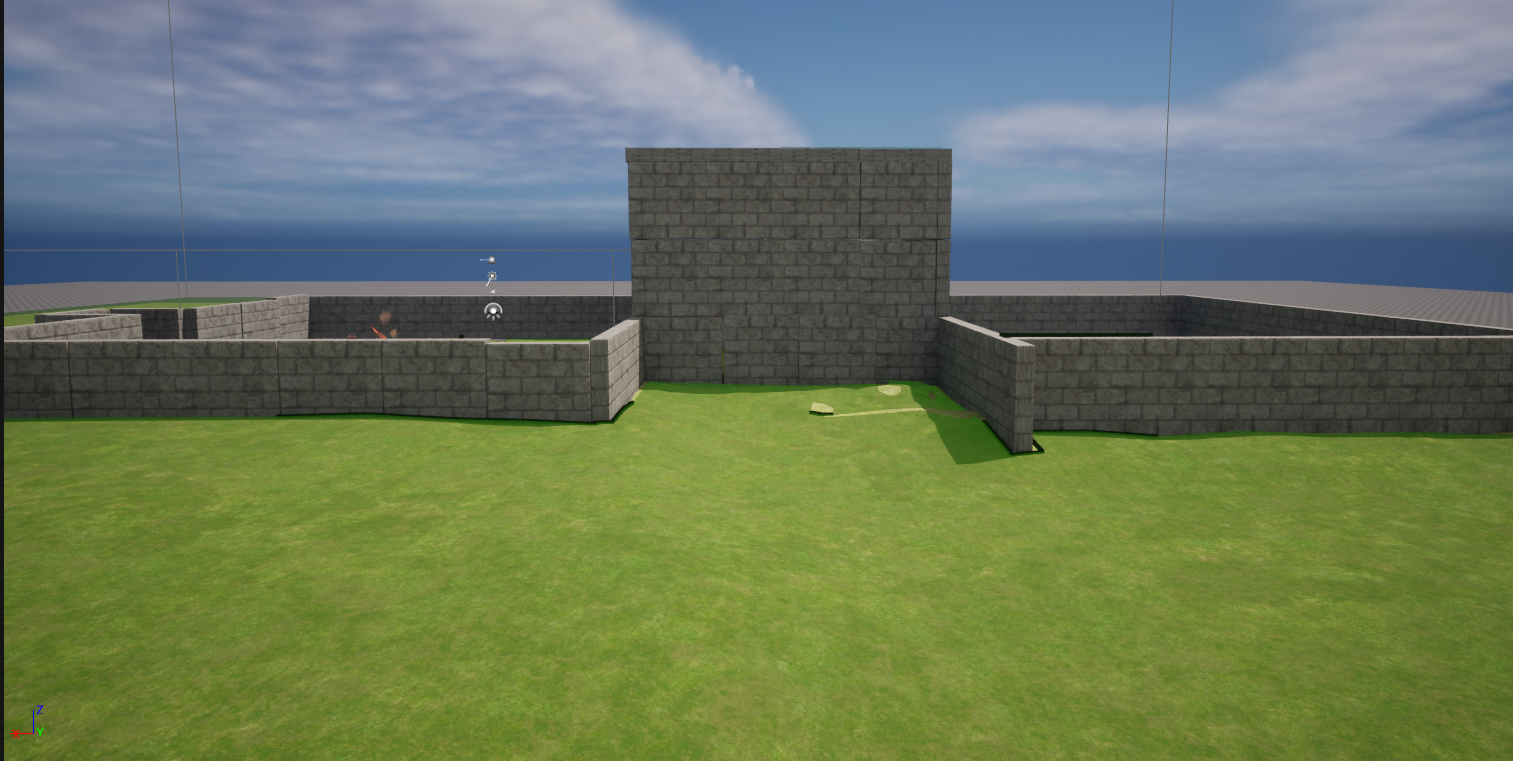
\includegraphics[width=6cm, height=6cm]{Figure/castle.png}\\ \\  
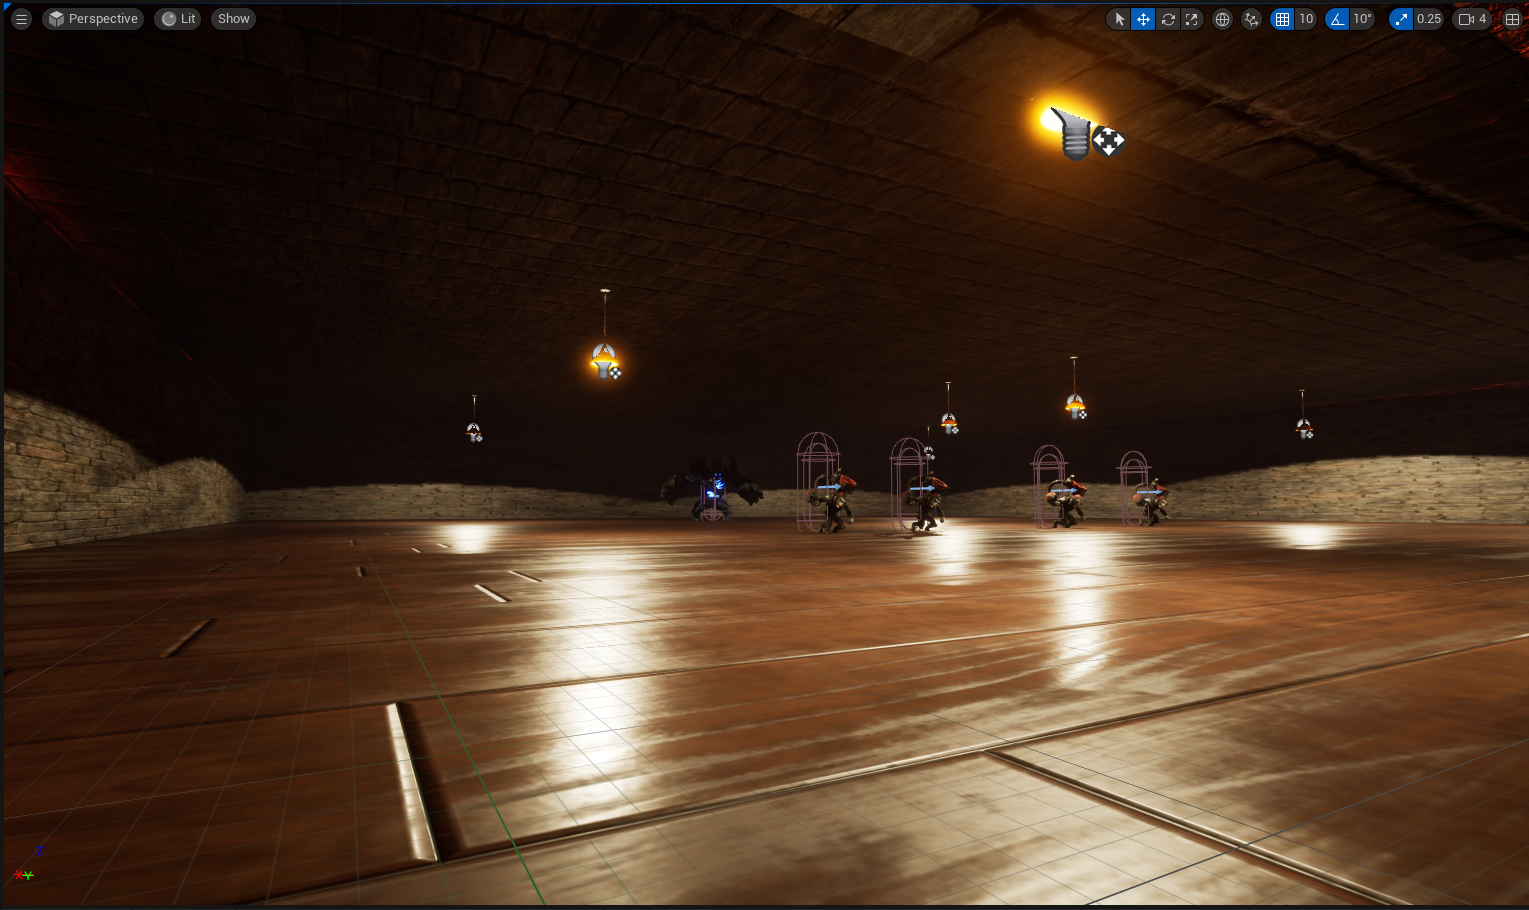
\includegraphics[width=6cm, height=6cm]{Figure/basement.png}\\ \\  
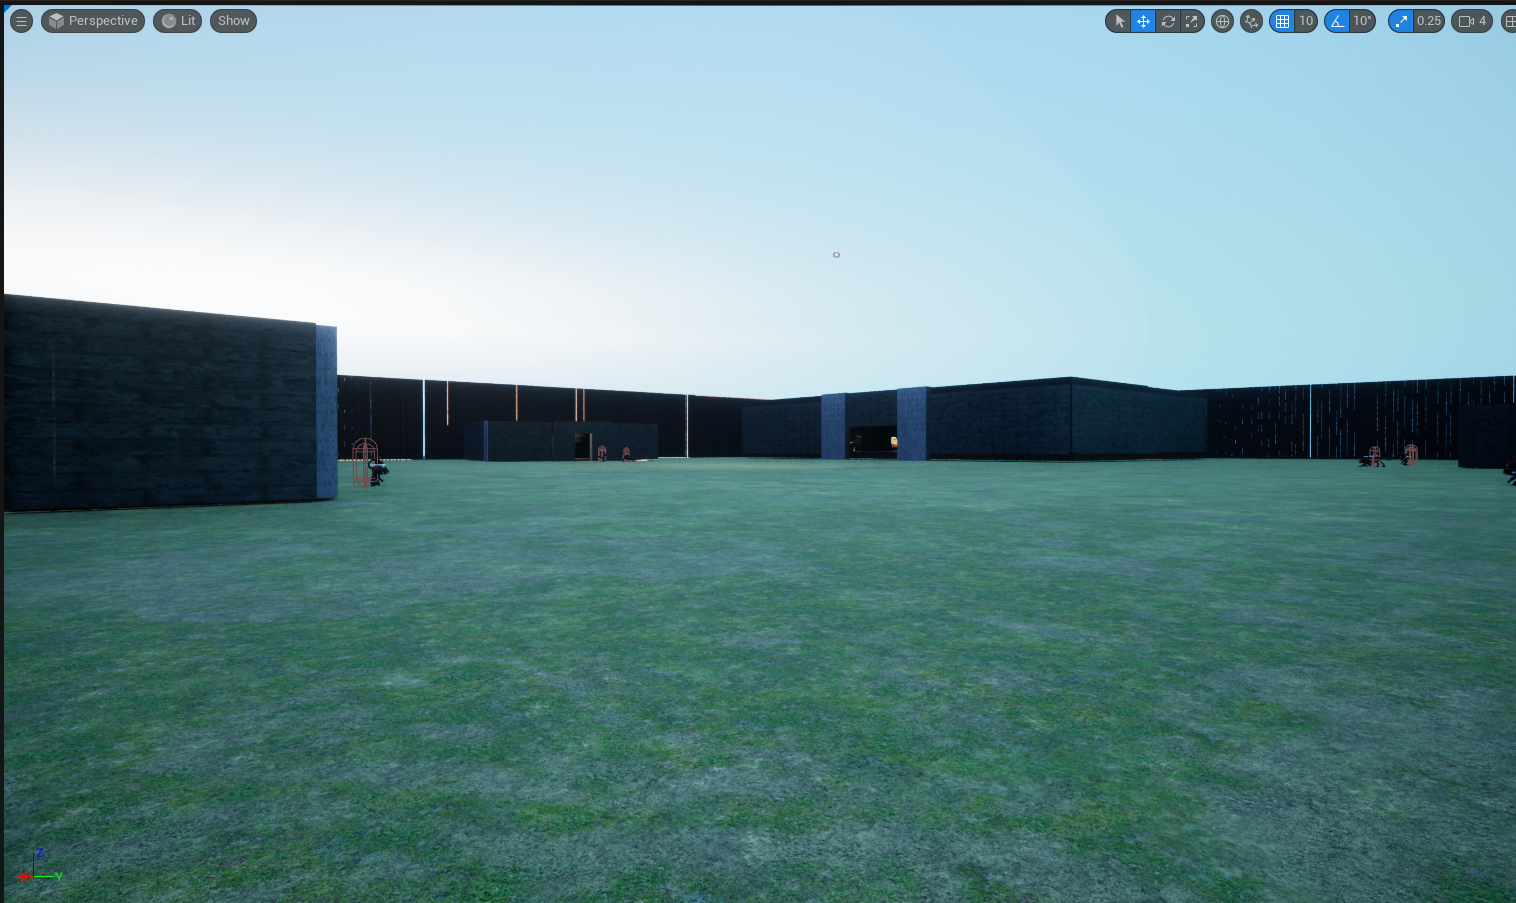
\includegraphics[width=6cm, height=6cm]{Figure/fort.png} \\ \\   

\section{Classes}
We made two classes for the game the mage and warrior.The warrior was the first class that was made and is the more simple of the two.Its first ability is just a heal ability which is useful for staying alive since you have to be in melee combat.The second ability is a damage buff which will give double damage to his attacks.The third ability is his ultimate which gives health regeneration to the player.The mage class is the range dps class.The first ability sends out fast moving disks in front of the player.The second ability shoots a fireball which does a lot for damage which is useful for the bosses in the game.The ult will regenerate  the players resources to cast more spells. \\
\includegraphics[width=6cm, height=6cm]{Figure/hammer.png}\\ \\   
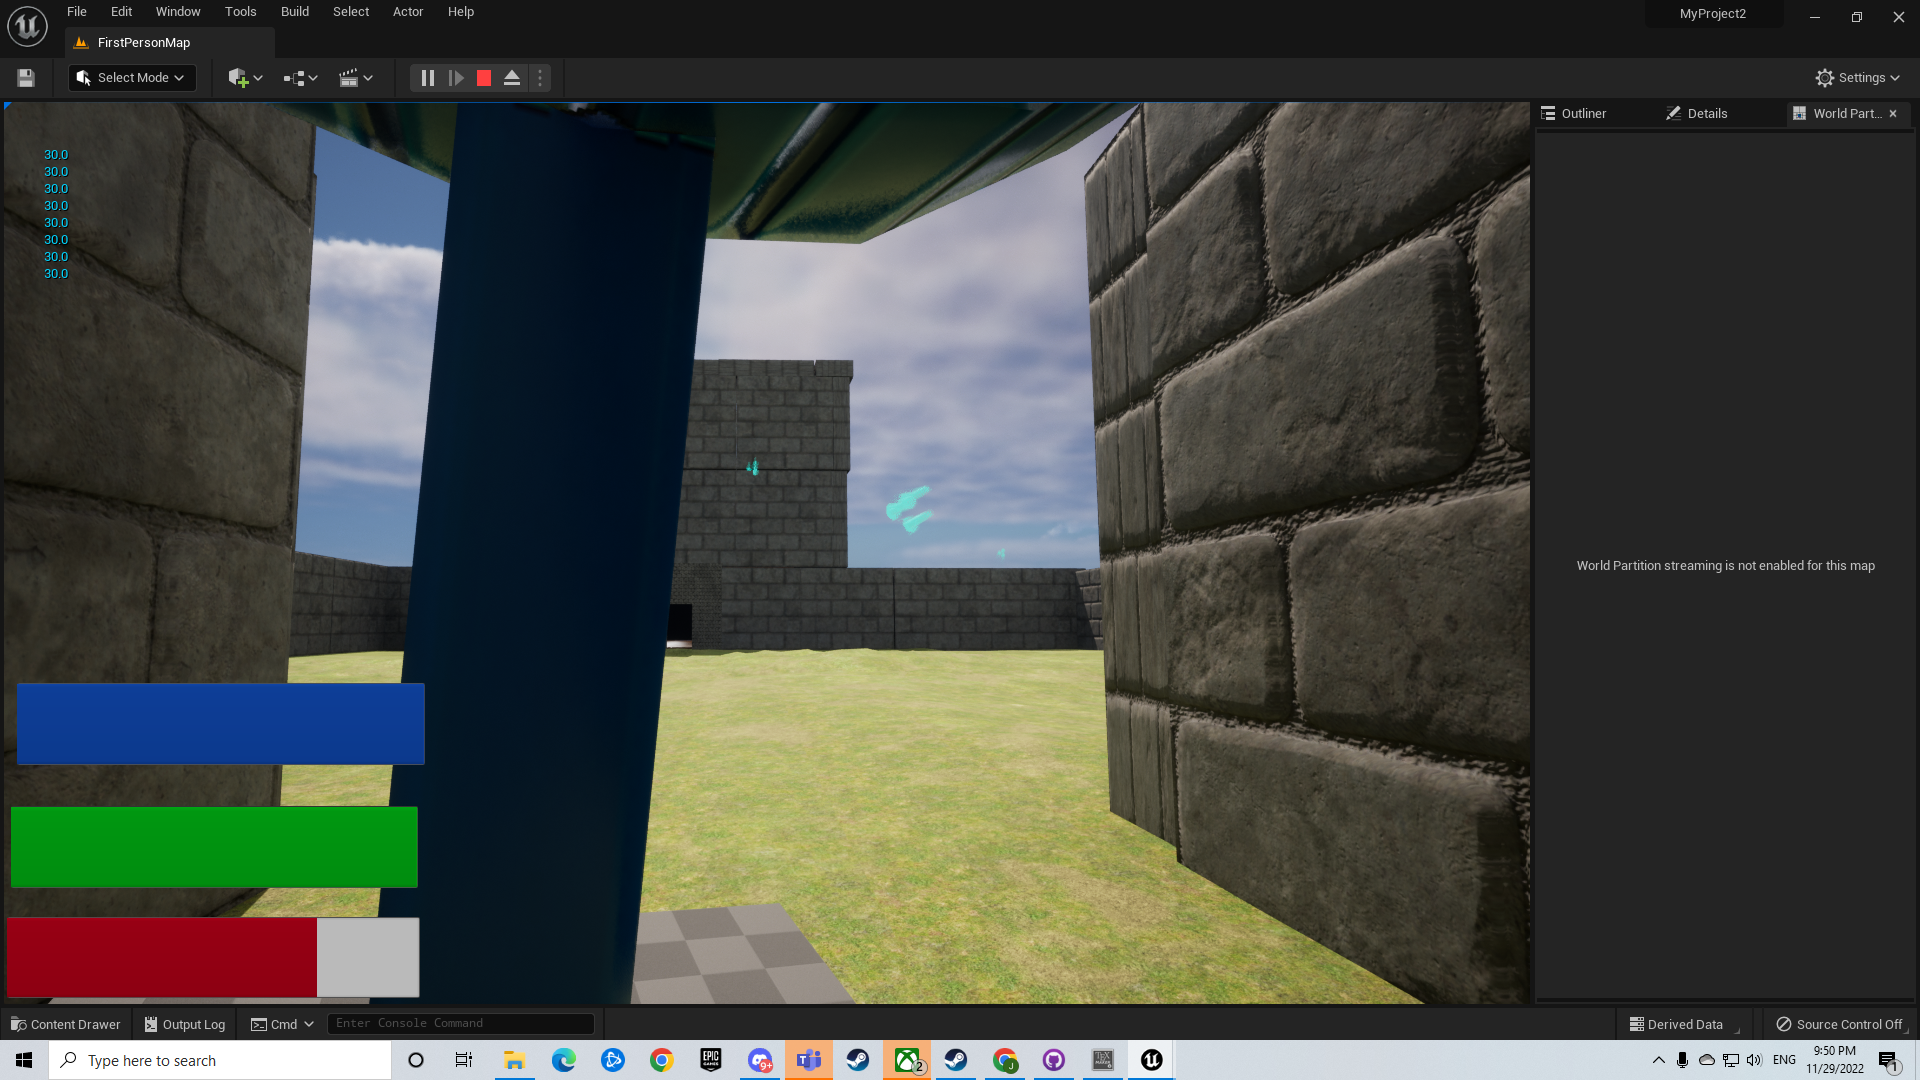
\includegraphics[width=6cm, height=6cm]{Figure/mage.png}\\ \\   
\section{What we learned}
This section will cover what we learned over the course of  making our project. Over the semester we learned about game development within unreal engine 5. Unreal engine is made by Epic Games and is free to use. We also learned how to go about making a game and all the steps that require it. Making the game involved a whole host of different things like having to plan out the different levels within the game, choosing an overall art direction for the game, deciding on what kind of enemies the player will go up against, and the different abilities the player character will have. Something else we learned how to do was create custom animations within the unreal engine. The enemies and their ai that is used to make them work was something else we learned. The player characters' different projectiles and weapons that can be used were implemented. An interface for the player character that shows the players health, magic, and ultimate ability was made. 

\section{mechanics}


\subsection{blueprints}
The major blueprints that were made were dealing with the classes.The projectiles used were changed blueprints of the original projectile.Things that were changed about it were the damage numbers gravity and speed.The class systems for the warrior used changing of simple variable values to achieve the effect of healing similar effects were done for other values such as resources and ultimate bars.The damage buff ability was achieved by having a damage buff variable  and having it change from 1 to 2 and having it affect weapon damage.The only problem I had with that was the casting to player character which took finding more information about casting online.
The mage abilities used similar blueprints since it was just spawning the projectile and the only thing that was different was the damage numbers and the cost in implementing.Overall the blueprints were very modular since you could reuse the code to do different abilities and projectiles.The ultimates were just having a timer run over different variable to regenerate that bar.\\
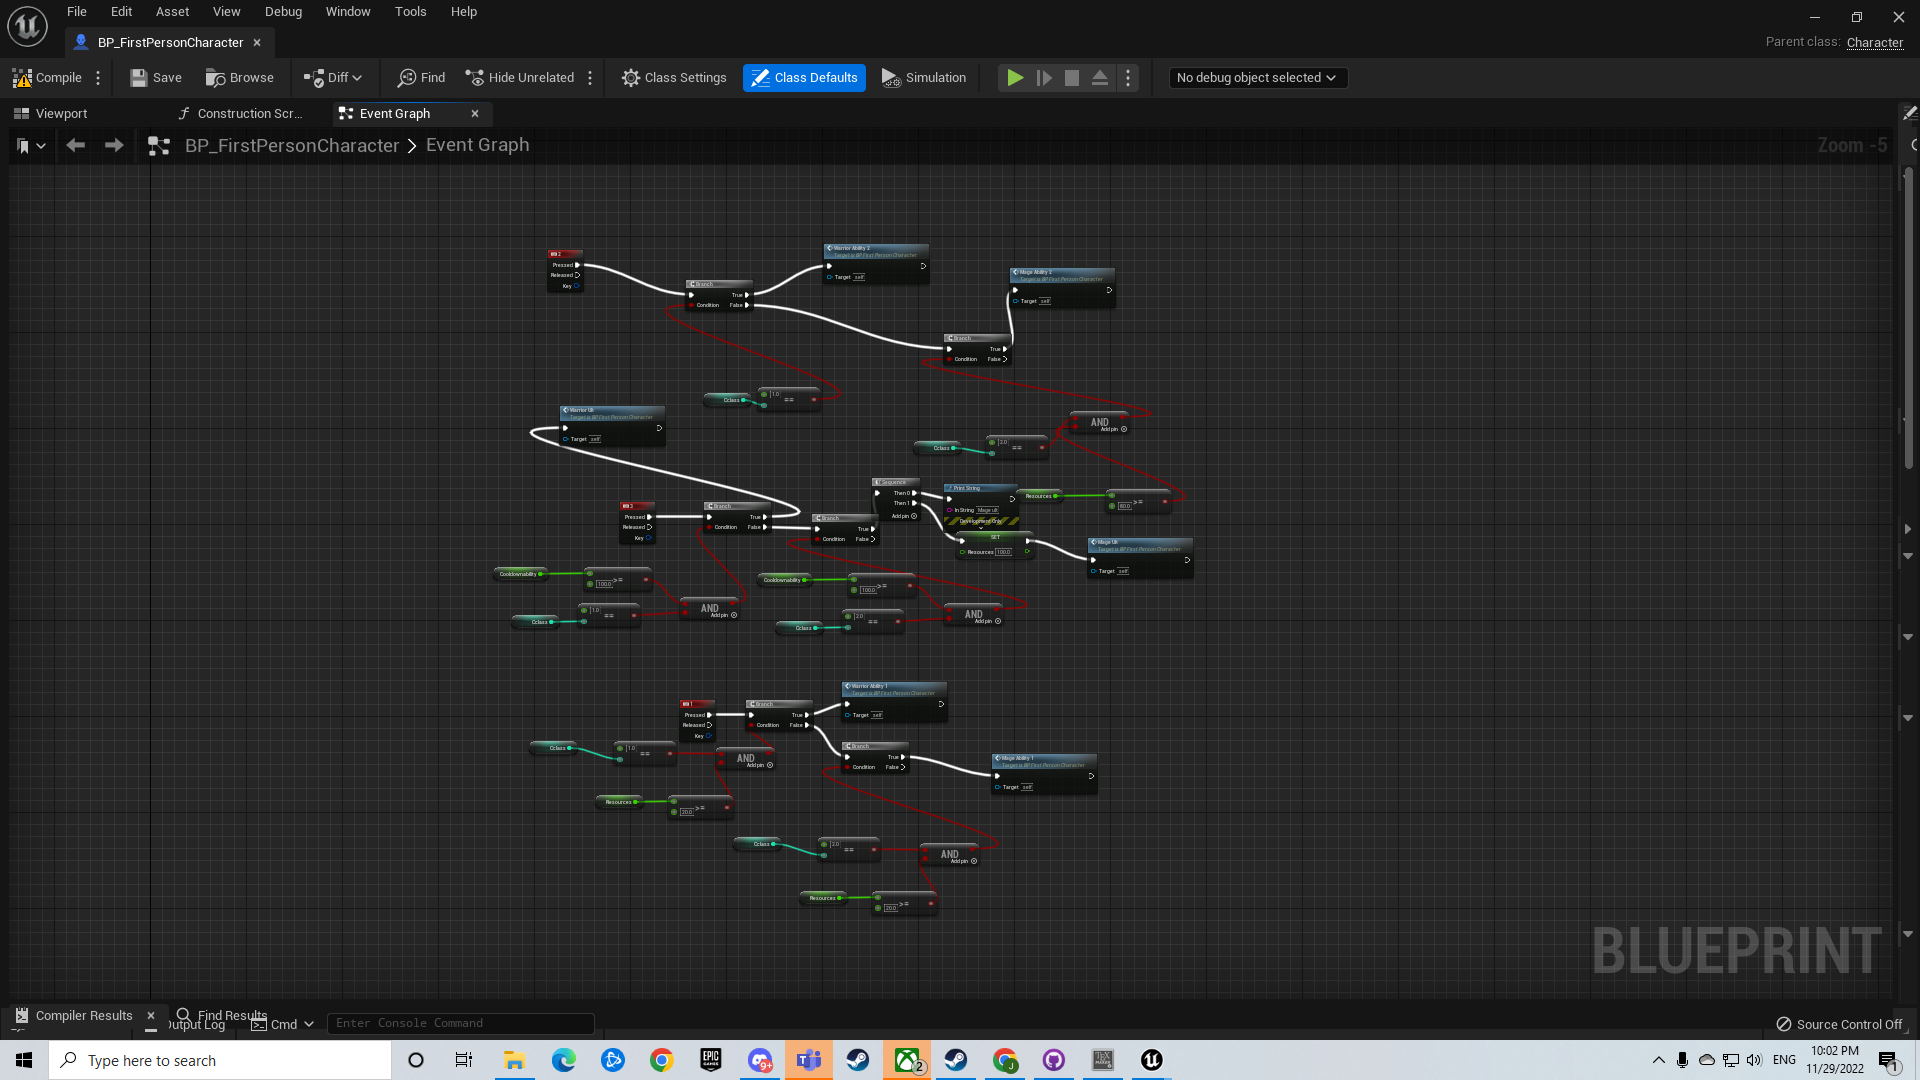
\includegraphics[width=6cm, height=6cm]{Figure/blueprint.png}\\ \\ 


\subsection{AI}
Ai was a little tricky since at first I just had simple blueprints to do basic tasks such as see and move towards the player.That later changed when I learned about behavior trees.All a behavior tree does is choose paths and execute commands.Example of commands used is turn to face player and walk towards player.The movement is basically  the ai finding a spot nearby and moving towards it until it sees the player.The AI will make the enemy move towards the player.This part of the project was difficult, and we had to use a tutorial made by unreal to get more information about behavior trees and get basic functionality. \\ 
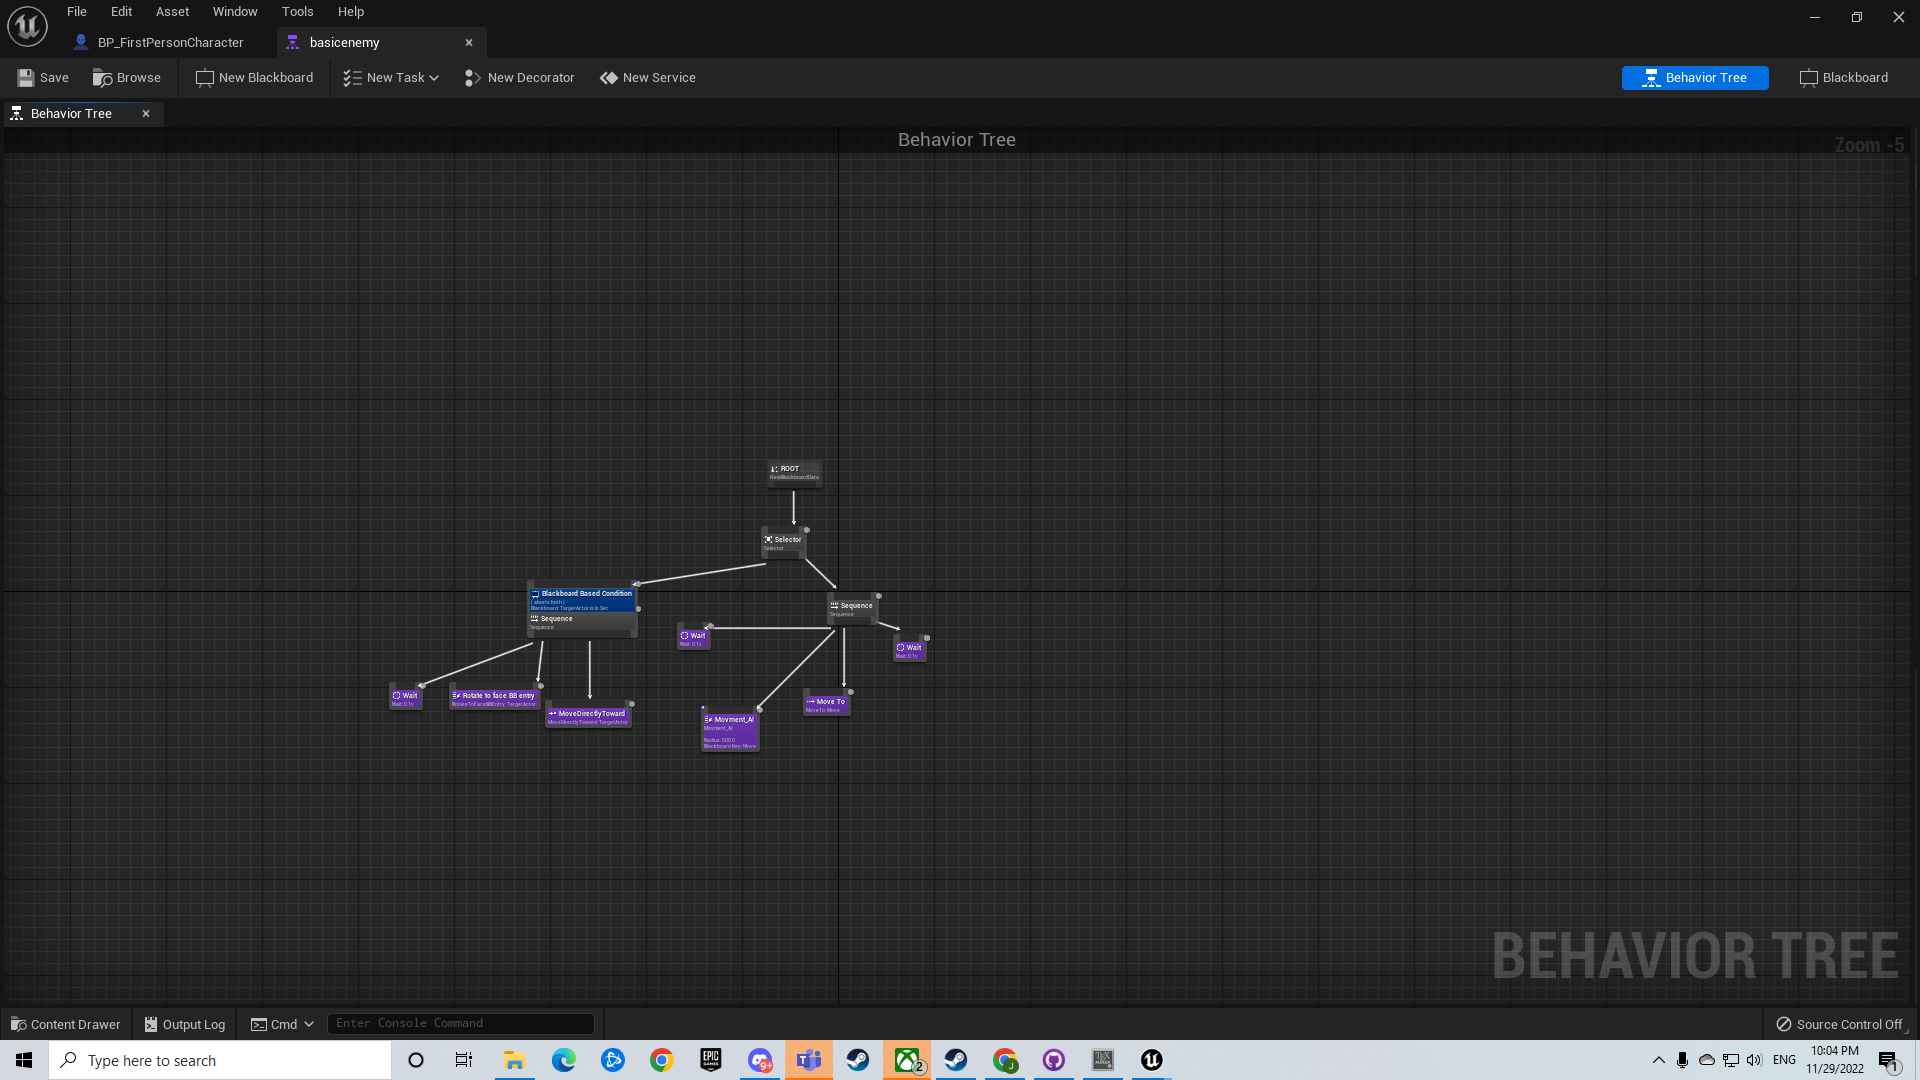
\includegraphics[width=6cm, height=6cm]{Figure/AI.png} \\ \\  

\section{Trials and Tribulations}
Over the course of creating and perfecting the project certain issues were encountered. Even though we used github for our version control and collaboration we still ran into using where work was lost. Another issue encountered was the differences in performance specifically gpu power between our personal machines complicated development.Some of the concepts were difficult such as the ai.There are also a lot of options on the blueprints and objects  so it was easy to get overwhelmed by it.Implementing the classes was tedious since choosing a class and a weapon can not be on the same keybind for some reason.The class ultimates were difficult since loops are awful in the blueprint system and would throw a no end condition error.We had to use timers which are much better to deal with. 


\section{Future Work}
There are some areas in our project that we weren't able to implement and could be considered future work. The first idea we had was porting the game to mobile. This is possible because unreal engines work cross platform. More levels being added was something else we would like to do in the future. Adding more enemies and weapons for the player character to use could also be worked on later down the road. 


\section{Project Development}
The project started with just a map that later became the empty castle.At first it was just messing with the toolkit to figure things out. I later added enemies that just stood there and then later they would move randomly.We started working on the second level which became the basement level since it seemed to transition well.The levels after the castle stay stagnant since we started to focus on the mechanics of the game.It first started with the ai which was a nightmare to work with so we switched over to working on the class system since it was easier.We added a warrior class with abilities such as healing, damage buff, and a regeneration ability.The ultimates required us learning about timers since they were required to make it work. The mage was the next class made which had different spells it could use.The spells required us to make more projectiles that have different stats.We then shifted focus back to the ai and got them to start moving round and attacking the player.Melee weapons were added close to the end of the project development.


\section{Opinions on Project}
The project was overall helpful for learning about a new toolkit and it forced me to look for help online when I ran into trouble.Example the ai was difficult since it required multiple blueprints and something called a black board.It also required making a ai controller for the enemies to use.We would have never figured that out unless we looked online for help.We also need to look up tutorials for the ai and the UI.Unreal does not really show you how to do things on its service.


\section{Conclusion}
To conclude over the semester with our project we were able to make a playable first person action game. This game was called the deep journey and was developed using unreal engine 5. We used the blueprint system within unreal engine 5 to deal with the different player classes and connect the levels using trigger boxes. The project development started out with just one level and by the end we had three distinct levels with different enemies the players could fit using their classes abilities. The project helped us learn game development and the new toolkits we needed to use. We have improvements and additions to the project that could be completed in the future. Overall this project was a fun way to demonstrate our resourcefulness/work ethic as computer science majors and showcases how we can use the knowledge we've procured over the years to accomplish great things. 



Your paper's title, authors and affiliations should run across the
full width of the page in a single column 17.8 cm (7 in.) wide.  The
title should be in Helvetica or Arial 18-point bold.  Authors' names
should be in Times New Roman or Times Roman 12-point bold, and
affiliations in 12-point regular.  

See \texttt{{\textbackslash}author} section of this template for
instructions on how to format the authors. For more than three
authors, you may have to place some address information in a footnote,
or in a named section at the end of your paper. Names may optionally
be placed in a single centered row instead of at the top of each
column. Leave one 10-point line of white space below the last line of
affiliations.

\subsection{Abstract and Keywords}

Every submission should begin with an abstract of about 150 words,
followed by a set of Author Keywords and ACM Classification
Keywords. The abstract and keywords should be placed in the left
column of the first page under the left half of the title. The
abstract should be a concise statement of the problem, approach, and
conclusions of the work described. It should clearly state the paper's
contribution to the field of HCI\@.

\subsection{Normal or Body Text}

Please use a 10-point Times New Roman or Times Roman font or, if this
is unavailable, another proportional font with serifs, as close as
possible in appearance to Times Roman 10-point. Other than Helvetica
or Arial headings, please use sans-serif or non-proportional fonts
only for special purposes, such as source code text.

\subsection{First Page Copyright Notice}
This template include a sample ACM copyright notice at the bottom of
page 1, column 1.  Upon acceptance, you will be provided with the
appropriate copyright statement and unique DOI string for publication.
Accepted papers will be distributed in the conference
publications. They will also be placed in the ACM Digital Library,
where they will remain accessible to thousands of researchers and
practitioners worldwide. See
\url{http://acm.org/publications/policies/copyright_policy} for the
ACM's copyright and permissions policy.

\subsection{Subsequent Pages}

On pages beyond the first, start at the top of the page and continue
in double-column format.  The two columns on the last page should be
of equal length.

%% \begin{figure}
%% \centering
%%   \includegraphics[width=0.9\columnwidth]{figures/sigchi-logo}
%%   \caption{Insert a caption below each figure. Do not alter the
%%     Caption style.  One-line captions should be centered; multi-line
%%     should be justified. }~\label{fig:figure1}
%% \end{figure}

\subsection{References and Citations}

Use a numbered list of references at the end of the article, ordered
alphabetically by last name of first author, and referenced by numbers
in
brackets.
Your references should be published materials accessible to the
public. Internal technical reports may be cited only if they are
easily accessible (i.e., you provide the address for obtaining the
report within your citation) and may be obtained by any reader for a
nominal fee. Proprietary information may not be cited. Private
communications should be acknowledged in the main text, not referenced
(e.g., ``[Borriello, personal communication]'').

References should be in ACM citation format:
\url{http://acm.org/publications/submissions/latex_style}. This
includes citations to internet
resources
according to ACM format, although it is often appropriate to include
URLs directly in the text, as above.


% Use a numbered list of references at the end of the article, ordered
% alphabetically by first author, and referenced by numbers in
% brackets~\cite{ethics, Klemmer:2002:WSC:503376.503378,
%   Mather:2000:MUT, Zellweger:2001:FAO:504216.504224}. For papers from
% conference proceedings, include the title of the paper and an
% abbreviated name of the conference (e.g., for Interact 2003
% proceedings, use \textit{Proc. Interact 2003}). Do not include the
% location of the conference or the exact date; do include the page
% numbers if available. See the examples of citations at the end of this
% document. Within this template file, use the \texttt{References} style
% for the text of your citation.

% Your references should be published materials accessible to the
% public.  Internal technical reports may be cited only if they are
% easily accessible (i.e., you provide the address for obtaining the
% report within your citation) and may be obtained by any reader for a
% nominal fee.  Proprietary information may not be cited. Private
% communications should be acknowledged in the main text, not referenced
% (e.g., ``[Robertson, personal communication]'').

\begin{table}
  \centering
  \begin{tabular}{l r r r}
    % \toprule
    & & \multicolumn{2}{c}{\small{\textbf{Test Conditions}}} \\
    \cmidrule(r){3-4}
    {\small\textit{Name}}
    & {\small \textit{First}}
      & {\small \textit{Second}}
    & {\small \textit{Final}} \\
    \midrule
    Marsden & 223.0 & 44 & 432,321 \\
    Nass & 22.2 & 16 & 234,333 \\
    Borriello & 22.9 & 11 & 93,123 \\
    Karat & 34.9 & 2200 & 103,322 \\
    % \bottomrule
  \end{tabular}
  \caption{Table captions should be placed below the table. We
    recommend table lines be 1 point, 25\% black. Minimize use of
    table grid lines.}~\label{tab:table1}
\end{table}

\section{Sections}

The heading of a section should be in Helvetica or Arial 9-point bold,
all in capitals. Sections should \textit{not} be numbered.

\subsection{Subsections}

Headings of subsections should be in Helvetica or Arial 9-point bold
with initial letters capitalized.  For sub-sections and
sub-subsections, a word like \emph{the} or \emph{of} is not
capitalized unless it is the first word of the heading.

\subsubsection{Sub-subsections}

Headings for sub-subsections should be in Helvetica or Arial 9-point
italic with initial letters capitalized.  Standard
\texttt{{\textbackslash}section}, \texttt{{\textbackslash}subsection},
and \texttt{{\textbackslash}subsubsection} commands will work fine in
this template.

\section{Figures/Captions}

Place figures and tables at the top or bottom of the appropriate
column or columns, on the same page as the relevant text (see
Figure~\ref{fig:figure1}). A figure or table may extend across both
columns to a maximum width of 17.78 cm (7 in.).

%% \begin{figure*}
%%   \centering
%%   \includegraphics[width=1.75\columnwidth]{figures/map}
%%   \caption{In this image, the map maximizes use of space. You can make
%%     figures as wide as you need, up to a maximum of the full width of
%%     both columns. Note that \LaTeX\ tends to render large figures on a
%%     dedicated page. Image: \ccbynd~ayman on
%%     Flickr.}~\label{fig:figure2}
%% \end{figure*}

Captions should be Times New Roman or Times Roman 9-point bold.  They
should be numbered (e.g., ``Table~\ref{tab:table1}'' or
``Figure~\ref{fig:figure1}''), centered (if one line) otherwise justified, and placed beneath the figure
or table.  Please note that the words ``Figure'' and ``Table'' should
be spelled out (e.g., ``Figure'' rather than ``Fig.'') wherever they
occur. Figures, like Figure~\ref{fig:figure2}, may span columns and
all figures should also include alt text for improved accessibility.
Papers and notes may use color figures, which are included in the page
limit; the figures must be usable when printed in black-and-white in
the proceedings.

The paper may be accompanied by a short video figure (we recommend staying within five
minutes in length). However, the paper should stand on its own without
the video figure, as the video may not be available to everyone who
reads the paper.  

\subsection{Inserting Images}
When possible, include a vector formatted graphic (i.e. PDF or EPS).
When including bitmaps,  use an image editing tool to resize the image
at the appropriate printing resolution (usually 300 dpi).

\section{Quotations}
Quotations may be italicized when \textit{``placed inline''}.

\begin{quote}
Longer quotes, when placed in their own paragraph, need not be
italicized or in quotation marks when indented.  
\end{quote}

\section{Language, Style, and Content}

The written and spoken language of SIGCHI is English. Spelling and
punctuation may use any dialect of English (e.g., British, Canadian,
US, etc.) provided this is done consis- tently. Hyphenation is
optional. To ensure suitability for an international audience, please
pay attention to the following:

\begin{itemize}
\item Write in a straightforward style.
\item Try to avoid long or complex sentence structures.
\item Use common and basic vocabulary (e.g., use the word ``unusual'' rather than the word ``arcane''.
\item Briefly define or explain all technical terms that may be
  unfamiliar to readers.
\item Explain all acronyms the first time they are used in your
  text---e.g., ``Digital Signal Processing (DSP)''.
\item Explain local references (e.g., not everyone knows all city
  names in a particular country).
\item Explain ``insider'' comments. Ensure that your whole audience
  understands any reference whose meaning you do not describe (e.g.,
  do not assume that everyone has used a Macintosh or a particular
  application).
\item Explain colloquial language and puns. Understanding phrases like
  ``red herring'' may require a local knowledge of English.  Humor and
  irony are difficult to translate.
\item Use unambiguous forms for culturally localized concepts, such as
  times, dates, currencies, and numbers (e.g., ``1--5--97'' or
  ``5/1/97'' may mean 5 January or 1 May, and ``seven o'clock'' may
  mean 7:00 am or 19:00). For currencies, indicate equivalences:
  ``Participants were paid {\fontfamily{txr}\selectfont \textwon}
  25,000, or roughly US \$22.''
\item Be careful with the use of gender-specific pronouns (he, she)
  and other gendered words (chairman, manpower, man-months). Use
  inclusive language that is gender-neutral (e.g., she or he, they,
  s/he, chair, staff, staff-hours, person-years). See the
  \textit{Guidelines for Bias-Free Writing} for further advice and
  examples regarding gender and other personal
  attributes~. Be particularly aware of
  considerations around writing about people with disabilities.
\item If possible, use the full (extended) alphabetic character set
  for names of persons, institutions, and places (e.g.,
  Gr{\o}nb{\ae}k, Lafreni\'ere, S\'anchez, Nguy{\~{\^{e}}}n,
  Universit{\"a}t, Wei{\ss}enbach, Z{\"u}llighoven, \r{A}rhus, etc.).
  These characters are already included in most versions and variants
  of Times, Helvetica, and Arial fonts.
\end{itemize}

\section{Accessibility}
The Executive Council of SIGCHI has committed to making SIGCHI
conferences more inclusive for researchers, practitioners, and
educators with disabilities. As a part of this goal, the all authors
are asked to work on improving the accessibility of their
submissions. Specifically, we encourage authors to carry out the
following five steps:
\begin{enumerate}
\item Add alternative text to all figures
\item Mark table headings
\item Add tags to the PDF
\item Verify the default language
\item Set the tab order to ``Use Document Structure''
\end{enumerate}
For more information and links to instructions and resources, please
see: \url{http://chi2016.acm.org/accessibility}.  The
\texttt{{\textbackslash}hyperref} package allows you to create well tagged PDF files,
please see the preamble of this template for an example.

\section{Page Numbering, Headers and Footers}
Your final submission should not contain footer or header information
at the top or bottom of each page. Specifically, your final submission
should not include page numbers. Initial submissions may include page
numbers, but these must be removed for camera-ready. Page numbers will
be added to the PDF when the proceedings are assembled.

\section{Producing and Testing PDF Files}

We recommend that you produce a PDF version of your submission well
before the final deadline.  Your PDF file must be ACM DL
Compliant. The requirements for an ACM Compliant PDF are available at:
{\url{http://www.scomminc.com/pp/acmsig/ACM-DL-pdfs-requirements.htm}}.

Test your PDF file by viewing or printing it with the same software we
will use when we receive it, Adobe Acrobat Reader Version 10. This is
widely available at no cost. Note that most
reviewers will use a North American/European version of Acrobat
reader, so please check your PDF accordingly.

\section{Conclusion}

It is important that you write for the SIGCHI audience. Please read
previous years' proceedings to understand the writing style and
conventions that successful authors have used. It is particularly
important that you state clearly what you have done, not merely what
you plan to do, and explain how your work is different from previously
published work, i.e., the unique contribution that your work makes to
the field. Please consider what the reader will learn from your
submission, and how they will find your work useful. If you write with
these questions in mind, your work is more likely to be successful,
both in being accepted into the conference, and in influencing the
work of our field.

\section{Acknowledgments}

Sample text: We thank all the volunteers, and all publications support
and staff, who wrote and provided helpful comments on previous
versions of this document. Authors 1, 2, and 3 gratefully acknowledge
the grant from NSF (\#1234--2012--ABC). \textit{This whole paragraph is
  just an example.}

% Balancing columns in a ref list is a bit of a pain because you
% either use a hack like flushend or balance, or manually insert
% a column break.  http://www.tex.ac.uk/cgi-bin/texfaq2html?label=balance
% multicols doesn't work because we're already in two-column mode,
% and flushend isn't awesome, so I choose balance.  See this
% for more info: http://cs.brown.edu/system/software/latex/doc/balance.pdf
%
% Note that in a perfect world balance wants to be in the first
% column of the last page.
%
% If balance doesn't work for you, you can remove that and
% hard-code a column break into the bbl file right before you
% submit:
%
% http://stackoverflow.com/questions/2149854/how-to-manually-equalize-columns-
% in-an-ieee-paper-if-using-bibtex
%
% Or, just remove \balance and give up on balancing the last page.
%
\balance{}

\section{References Format}
Your references should be published materials accessible to the
public. Internal technical reports may be cited only if they are
easily accessible and may be obtained by any reader for a nominal
fee. Proprietary information may not be cited. Private communications
should be acknowledged in the main text, not referenced (e.g.,
[Golovchinsky, personal communication]). References must be the same
font size as other body text. References should be in alphabetical
order by last name of first author. Use a numbered list of references
at the end of the article, ordered alphabetically by last name of
first author, and referenced by numbers in brackets. For papers from
conference proceedings, include the title of the paper and the name of
the conference. Do not include the location of the conference or the
exact date; do include the page numbers if available. 

Citing something\cite{unrealweb}. \cite{wizard} \cite{infinityw} \cite{infinitya}


% BALANCE COLUMNS
\balance{}

% REFERENCES FORMAT
% References must be the same font size as other body text.
%%\bibliographystyle{SIGCHI-Reference-Format}
%% \bibliographystyle{acm-sigchi-proceedings}

\bibliographystyle{plain}
\bibliography{bibliography}

\end{document}


